\chapter{Analog Digital Converter}

In this chapter two different versions of our ADC are getting described.

\section{Idea}

The task was to implement an 16bit ADC. We decided to implement a tracking ADC, the idea is shown in Figure ~\ref{fig:wholeADC}. This kind of ADC has different advantages, e.g. that it is choosable how good the approximation is by setting the correct frequency of the clock. Also it matches the requirements of using the DAC and the OpAmp. Our ADC is linear to the input value, which means, you can multiply the digital value with an fixed value, which depends on V\textsubscript{dd}, to get an approximation of the input value. E.g. if you are using 1.2V as V\textsubscript{dd}, you can calculate 

\begin{equation}
	V_{approx} = \frac{1.2V}{2^{16} - 1} \cdot digitalValue
\end{equation}

to get the approximation of the input.

\begin{figure}[h]
	\centering
	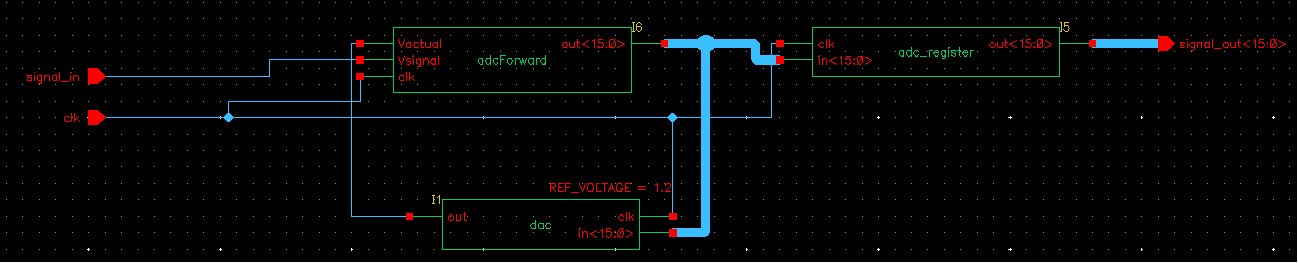
\includegraphics[scale=0.5]{images/adc/adc.png}
	\caption{the high-level view of the ADC}
	\label{fig:wholeADC}
\end{figure} 

There were several problems encountered while implementing the ADC. Besides of performance problems of Cadence, which resulted into a slow down of the development process, the comparator misses differences at its input stages, when they are to small. This results into the fact, that the ADC is not working at a stepwidth of one, but maybe at a stepwidth of 100. If the difference at the input stage of the comparator is to small, it does not return a digital value, but something in between. To face this problem, you could use several stages of comparators, but we decided to use just one stage, to show the principial, and afterwards some ideal Verilog-A modules called \texttt{simpleADC} and \texttt{simpleADCExtended}. 

\section{First Implementation}

The first implementation uses a stepwidth which has to be choosen by the user before the ADC starts to work. This has the advantage of simplifying the ADC because it does not need a stepwdith control but it is also not able to adapt to different stepwidths. This one should be used, when the analog input is nearly known and the stepwidth should be choosen carefully.

\subsection{Design}

The interesting part of the design is the part of the ADC called ADCForward. This first implementation of the forward path is shown in figure ~\ref{fig:simpleForward}. You can see that in the first step it gets decided, if the counter shall count up, down or stall. This information gets into the counter, which processes the runtime information and uses the previous configured stepwidth, to calculate the next value. As you can see in ~\ref{fig:wholeADC} this new value gets through a feedback path, containing a DAC, back to the forward path and the first part of the forward path can decide again, if the actual value is to high, so count down, to low, so count up or matching, so stop counting.

\begin{figure}[h]
	\centering
	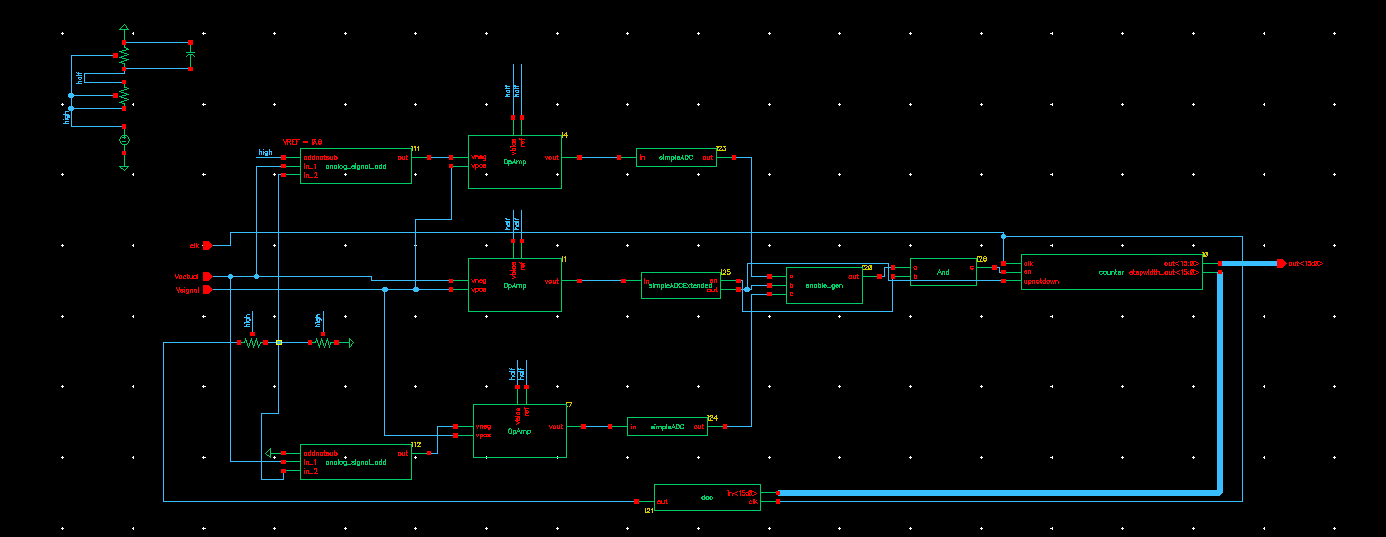
\includegraphics[scale=0.45]{images/adc/adcForward.png}
	\caption{the simple adc forward path}
	\label{fig:simpleForward}
\end{figure}

\subsection{Evaluation}

As result of the evaluation task, we got the diagram provided in figure ~\ref{fig:simpleAdcEvaluation}, using a stepwidth of 4500. The requested values can be found at table ~\ref{table:valuesSimpleADC}. Due to Cadence performance problems, the differential and integral non-linearity (DNL/INL) of the ADC could not be evaluated.

\begin{figure}[h]
	\centering
	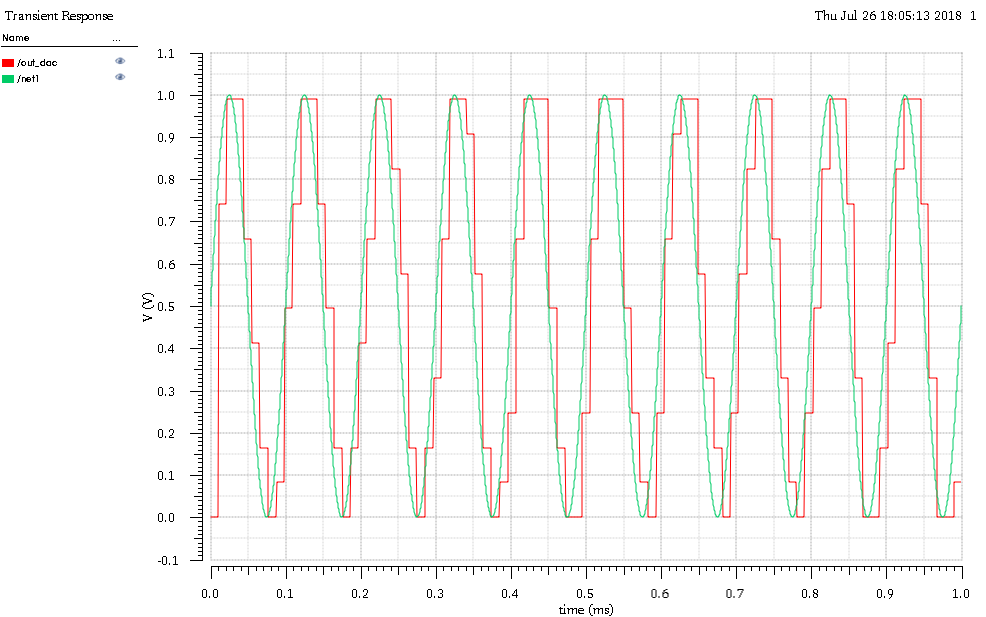
\includegraphics[scale=0.5]{images/adc/10KHzInputStepWidth4500.png}
	\caption{10kHz input and stepwidth 4500}
	\label{fig:simpleAdcEvaluation}
\end{figure}

\begin{table}[!h]
	\centering
	\begin{tabular}{|l|l|}
		\hline
		Name & Value \\
		\hline
		Maximal Sampling Frequency & 100kHz \\
		ENOB & 1.576225 bits \\
		SINAD & 11.251875 dB \\
		SNR & 11.251875 dB \\
		\hline
	\end{tabular}
	\caption{values of the simple ADC}
	\label{table:valuesSimpleADC}
\end{table}

\section{Second Implementation}

The second implementation does not need to get a stepwidth, but calculates its own stepwidth at runtime. It is more complex, but usefull, if you do not know anything about the incoming signal.

\subsection{Design}
Also here, the interesting part of the ADC is the forward path, which is called ADCForwardExtended here. This second implementation is shown in figure ~\ref{fig:extendedForward}. You can see that this forward path is divided in three steps. First, new stepwidths are getting calculated from the last choosen stepwidth. After that, the new possible values are computed and the stepwidth chooser selects the one, which is fitting best. It is also possible that the stepwdith chooser decides, that none of them are fitting good, so it keeps the last digital value and returns as used stepwidth zero.

\begin{figure}[h]
	\centering
	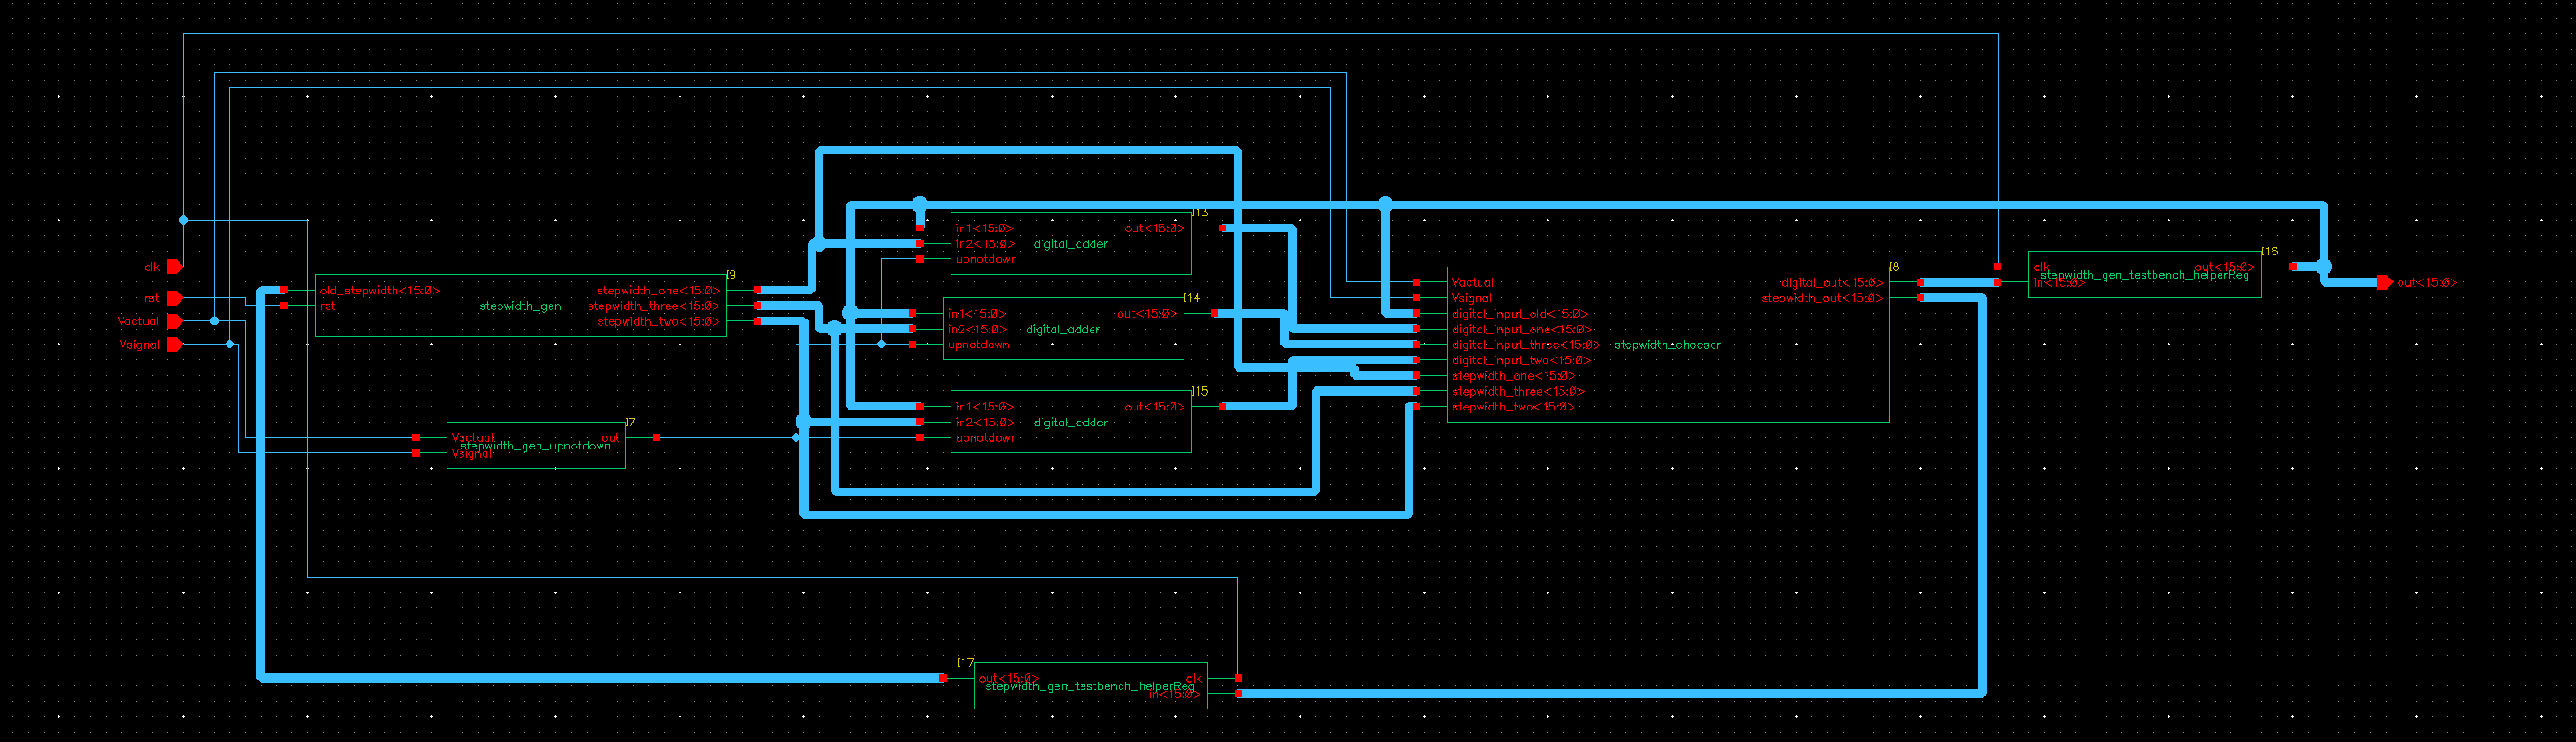
\includegraphics[scale=0.225]{images/adc/adcForwardExtended.png}
	\caption{the extended ADC forward path}
	\label{fig:extendedForward}
\end{figure}


\subsection{Evaluation}

The simulation results are shown in figure ~\ref{fig:extendedAdcEvaluation}. The requested values can be found at table ~\ref{table:valuesExtendedADC}, but here again, INL and DNL could not be computed.


\begin{figure}[h]
	\centering
	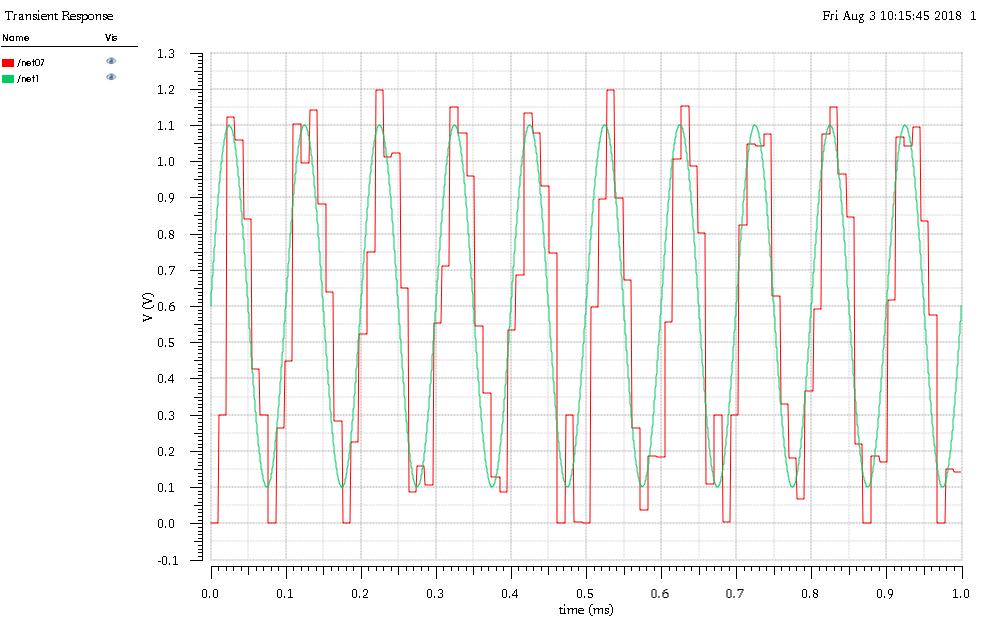
\includegraphics[scale=0.5]{images/adc/input10kHzExtended.png}
	\caption{10kHz input for the extended ADC}
	\label{fig:extendedAdcEvaluation}
\end{figure}

\begin{table}[!h]
	\centering
	\begin{tabular}{|l|l|}
		\hline
		Name & Value \\
		\hline
		Maximal Sampling Frequency & 100kHz \\
		ENOB & 1.7770844 bits \\
		SINAD & 12.461048 dB \\
		SNR & 12.461048 dB \\
		\hline
	\end{tabular}
	\caption{values of the extended adc}
	\label{table:valuesExtendedADC}
\end{table}